\documentclass[../main.tex]{subfiles}

\begin{document}


\section{Estimation}

\subsection{Data Moments}
\label{sec:moments}

Having explored both our theoretical framework and the data we have on sick leaves, we turn to calibrating our ``implicit'' search model using that data. Our main blind spot is the fact that we have no information on overall patient visits by each physician ($Q_j$), only the sick leaves they were authorized to issue in the sampled period ($X_j$). We get the necessary variation to be able to identify and estimate our parameters from two sources: by assigning each of the 48,611 physicians to one of ten equally sized ``quality'' bins (or decile ranks) and by making a distinction between overall sick leaves granted and those of 30 days or more.

A qualitative consequence of both our proposed models is that physician strategies $\bar{\kappa_j}$ were growing on physician ``quality'' $V_j$, or alternatively put, ``strictness'' decreasing on $V_j$, meaning that as physicians expect less and less demand from their own reputation as medical professionals, they would adjust by acquiring a reputation as lenient sick leave issuers. This behavior, not an analytical given from our framework, holds for our proposed distributions for $F(\kappa)$ and $G(\gamma)$.

Being that we lack data on observable qualities from physicians, including individual salary and educational background, our approach to grouping them into quality bins was to make use of that observed relationship and its corollary: higher quality physicians will raise their threshold $\bar{\kappa_j}$ and thus see patients of higher $\kappa_i$ on average, and in particular, a higher proportion of their patient base will be composed of patients satisfying $\kappa_i > \bar{\kappa}_{\max}$.

In this regard we can make use of the intensive margin of the sick leaves in our data, namely that we know their \textit{duration} (in days). We argue that the population equivalent of patients whose $\kappa_i > \bar{\kappa}_{\max}$ is patients who received sick leaves of 30 or more days. Though in a sense an arbitrary threshold, it so happens that starting at 30 days sick leaves are subject to higher institutional scrutiny and are automatically sent to the overseeing authority, subject to their authorization, requiring some medical proof—a test result—of the patient's ailment. At that point, the possibility of outright fraud can be safely discarded.

From a medical standpoint, a condition which would require a leave of absence of 30+ days is serious enough that no competent medical professional would wave off entirely the necessity for rest. This is to say, for a given authorized sick leave of 30+ days in our sample, we could reasonably picture that a ``stricter'' physician would have signed for less days off, say, just two weeks, but it is out of the question that, agreeing on diagnosis, what one physician considers as requiring over a month off work the other would not even consider as warranting any sick leave at all.

Figure \ref{fig:cdf} illustrates the empirical cumulative distribution of sick leave durations across all observations in our dataset.\footnote{Since this probability distribution assumes integer values only, the cumulative probability of a sick leave lasting 30 or more days is calculated as $1 - \text{CDF}(29)$.} Sick leaves lasting 30 days or more account for 20.05\% of issuances during the sample period. In particular, sick leaves of exactly 30 days represent 15.64\% of the total, a significant discrete jump in the curve which afterwards becomes almost flat. The highest duration of any single sick leave within our sample is 728 days.

\begin{figure}[H]
    \centering
    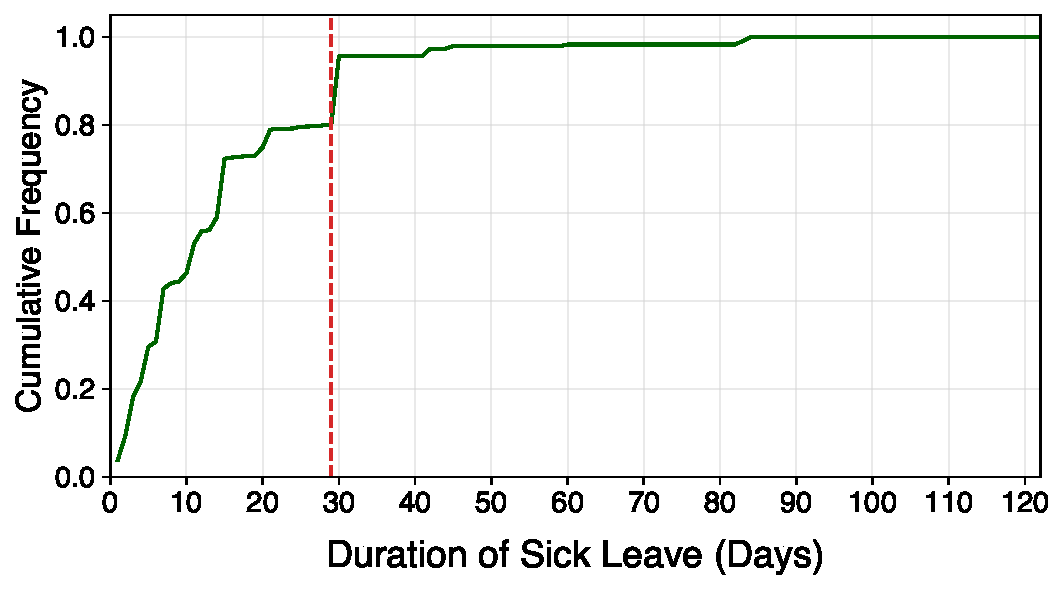
\includegraphics[width=0.70\linewidth]{cdf.pdf}
    \captionsetup{justification=centerlast}
    \caption{Empirical cumulative distribution of sick leave durations. \\ A red dashed line is placed at 29 days.}
    \label{fig:cdf}
\end{figure}



We first make use of this distinction to set up our physician quality bins. We design a \textit{quality score} variable by physician based on the three following criteria:
\begin{enumerate}[label=\roman*, itemsep=0pt, topsep=0pt]
    \item Average duration of sick leaves issued.
    \item Percentage of sick leaves of 30+ days over total in sampled period.
    \item Amount of sick leaves of 30+ days issued.
\end{enumerate}

The quality bin to which a physician is assigned corresponds to the decile rank of \textit{quality score} to which they belong. See Appendix \ref{sec:par} for a breakdown of the construction of the score variable and the physician bins.

This procedure does perhaps amount to an over-exhertion of our data sample, recognizing that by taking qualitative results from our model as a presumed basis we somewhat pre-fit our data to the model even before calibration, but it is by no means an econometrically unsanctioned manouver, as the population moments with which we calibrate our parameters contain, in part, different information to that with which we set up the bins themselves, so that identification is in fact possible. 

It would indeed be best to assign a quality score based on a set of observables wholly separate from those which play the role of endogenous outcomes in our model, but our course of action is sufficient for our purpose, which isn't to \textit{falsify} our framework—built upon observations and findings established in the relevant literature—but to showcase it and present an approach for its estimation.

Our second use of the distinction between overall sick leaves and the `30+ days' subsample is that we use both as data moments to calibrate our parameters. This means we have two moments \textit{per} quality bin, 20 moments in total, to fit our model, as we won't consider variation across the $r_j$ or $\tau_j$ axes.

To define both moments formally within our framework, each bin corresponds to a representative physician $j$, where $J = 10$, such that we have two $J$-dimensional vectors, $X$ and $X^{30}$, where the $j$th component of each corresponds respectively to the two following moments for representative physician $j$:
\begin{align}
    X_j \,=\, &  \int_{\bar{\kappa_j}}^{\infty} \int_{0}^{\infty}s_{ij}(\kappa, \gamma)  \,dG(\gamma) \,dF(\kappa) \tag{\ref{eq:s_X}}
\end{align}
\begin{align}
    X_j^{30} \,=\, & \int_{\bar{\kappa}_{\max}}^{\infty} \int_{0}^{\infty}s_{ij}(\kappa, \gamma)  \,dG(\gamma) \,dF(\kappa)
    \label{eq:X30}
\end{align}

The advantage of using this second defined moment, $X^{30}$, lies in its independence from the choice of strategy $\bar{kappa_j}$ and its \textit{near} independence from the distribution $G(\gamma)$. Any patient satisfying $\kappa_i > \bar{\kappa}_{\max}$ will, by definition, be granted sick leave by any physician. The implication of this on the probability $s_{ij}$ that such a patient visits any physician $j$ can be seen as follows:
\begin{align*}
    s_{ij} = \frac{\alpha_{ij}}{\sum_{k = 1}^{J} \alpha_{ik}} & =
    \frac{e^{\lambda u_{ij}}}{\sum\limits_{k : \; u_{ik} \geq 0} \hspace{-0.5em} e^{\lambda u_{ik}}} 
    =
    \frac{e^{\lambda \{V_j \kappa_i + \gamma_i - \tau_j \}}}{\sum\limits_{k : \; u_{ik} \geq 0} \hspace{-0.5em} e^{\lambda \{V_k \kappa_i + \gamma_i - \tau_k \}}} \\
    \\ 
   & = \frac{e^{\lambda \{V_j \kappa_i - \tau_j \}} \cancel{e^{\lambda \gamma_i}}}{\sum\limits_{k : \; u_{ik} \geq 0} \hspace{-0.5em} e^{\lambda \{V_k \kappa_i  - \tau_k \}} \cancel{e^{\lambda\gamma_i}}} =
    \frac{e^{\lambda \{V_j \kappa_i - \tau_j \}}}{\sum\limits_{k : \; u_{ik} \geq 0} \hspace{-0.5em} e^{\lambda \{V_k \kappa_i - \tau_k \}}}
\end{align*}

We see that $\gamma_i$ can be factored out of the defining fraction. It still plays a role, however, in the condition of the summation in the denominator. Physicians afforded a strictly positive probability of visit by patient $i$ must meet the $u_{ij} \geq 0$ condition implied by our \textit{free disposal} patient rationality. This in turn requires of one such physician $j$ to fulfill $V_j \kappa_i + \gamma_i \geq \tau_j$. So the scale of $\gamma_i$ still has implications for $X^{30}$ in this regard, only insofar as it may take a physician completely out of rotation for a patient's strategy vector $S_i$. We can see in the Appendix \ref{sec:id} that the moment outcomes of our model fit are much less responsive to variations in the parameters for $G(\cdot)$ in the case of $X^{30}$ as in overall $X$.


\subsection{Parameters and Estimation Results}

There are several elements in this model that require specification and then calibration. Starting with the two population distributions $F(\kappa)$ and $G(\gamma)$ describing patients, in keeping with their analogues in \cite{schnell2017physician}, we choose an exponential distribution for $\kappa$ with a $\lambda_F$ scale parameter, such that as ``medical necessity'' (`pain severity' in Schnell) grows larger , it becomes increasingly rare — whereas for $\gamma$, the ``taste for sick leave'' (for prescription drugs in Schnell), we choose a normal distribution, parametrized by a mean $\mu$ and variance $\sigma$.

Both $\mu$ and $\sigma$ we will fit through calibration, but for $\lambda_F$ we simply normalize it to 2, in order to have the average $\kappa_i$ in the population be $1/2$, on aesthetic grounds. We normalize $\lambda_F$ because it couldn't otherwise be correctly identified, as $\kappa_i$ only ever appears in the patients' utility function accompanied by a multiplying $V_j$. Being the case that we will calibrate the values of $V_1$ through $V_{10}$, we need to fix a value for the distribution of $\kappa$, else identification will fail. Fortunately for us, and not coincidentally, what matters really is the shape of the distribution. Given the \textit{scaling property} of the exponential distribution, if some value $k^*$ is the true population parameter for $\lambda_F$, rather than 2, then the ``true'' values for the components of the physician quality vector $\vec{V}$ would follow $V_j^* = 2/k^* \; V_j$. But then the accompanying expected value of $\kappa_i$ would itself be scaled by $k^*/2$, such that for these \textit{true} values the level of each $V_j \kappa_i$ would remain as before. Given that only this single term $V_j \kappa_i$ is relevant to inform agent behavior, not each product individually, in the end our choice of $\lambda_F$ makes no difference.

As for physicians, as we mentioned, we will estimate the ten components of the $\vec{V}$ vector. With respect to their utility function, the form we give to the revenue and punishment functions, $R_j(\cdot)$ and $P(\cdot)$, is a linear function $r_j Q_j$ and a strictly convex quadratic function $p / 2 \cdot (X_j)^2$. For convenience, we will disregard the $j$ subscript in the revenue function like we have done all along for $P(\cdot)$. The parameter $p$ will be subject to GMM estimation, whereas $r$—and for that matter the cost of visit $\tau_j$, which shall also be the same $\tau$ for all physicians—we obtain from the data directly, doing a weighted average of listed prices for doctor visits by FONASA matched with the 10 most common conditions granted sick leave. The resulting values for $r$ and $\tau$ are 21.182 and 8.944, respectively. See Appendix \ref{sec:par} for more detail on the calculation.

The choice of a linear function for $R_j(\cdot)$ is natural and precedented, the parameter $r_j$ ($r$) has a direct interpretation as the revenue by visit for physician $j$. The choice of $P(\cdot)$ is a little more subtle. At this point we would like to point out, it is not self-evident that our \textit{punishment} function should take total sick leaves granted by physician ($X_j$) as its argument. The reasoning behind it is the fact that the patients' $\kappa_i$ would be unobservable to the institutional overseer, as is the case in the real-life setting, where reports on the patients' conditions come in most cases from the very same agent that issues sick leaves, the physician, making fraud and misdiagnosis be undetectable in these instances.

As a crutch, institutional discipline relies on what variables \textit{are} observable, namely, the amount of sick leaves issued within a given period by physician. As chronicled by \cite{oteiza}, in 2021 the regulatory authority COMPIN sanctioned a subsample of physicians who were eggregious outliers in their volume of sick leaves issued and were unable to justify it. The `expected punishment' which faces some physician $j$ could be formalized as:
\[
\text{fine\_\$} \times \operatorname{Pr}[\text{fined} \mid X_j]
\]
The probability of being find would be near 0 until $X_j$ gets to be above around the 90th percentile, at which point it starts steadily increasing. If we allowed the magnitude of the fine to increase in proportion to the level of $X_j$, the `punishment function' would be more convex still. We choose $p / 2 \cdot (X_j)^2$ as a reasonable polynomial approximation of the function implied by our description. Convexity would not be nearly as steep as described, but it has the advantage of parsimony. The parameter $p$ then takes on the interpretation of both magnitude and probability of fine, anything that impacts the expected punishment physicians envisage for any given level of $X_j$.

\begin{table}[H]
    \centering
    \small
    \begin{tabular}{lcc}
        \toprule
        Parameter  & Value & Source \\
        \midrule
        Physician quality bins && \\
        \hspace{1em}$V_1$ ... $V_{10}$ & $\vec{V}_{1 \times 10}$ & GMM \\
            \\
        Punishment function $P(\cdot)$ && \\
            \hspace{1em}$p$ & 1.953 &  GMM\\
            \\
        Medical need distribution $F(\kappa)$ && \\
            \hspace{1em}$\lambda_F$ & 2 & \hspace{0.25em} Normalization\\
            \\
        Taste distribution $G(\gamma)$ \\
            \hspace{1em}$\mu$ & 73.997 &  GMM\\
            \hspace{1em}$\sigma$ & 18.492 &  GMM\\
            \\
        Logit model parameter && \\
            \hspace{1em}$\lambda_s$ & 0.842 & GMM\\
            \\
        Maximum threshold level && \\
            \hspace{1em}$\bar{\kappa}_{\max}$ & 0.763 &  GMM\\
            \\
        Revenue/cost of visit && \\
            \hspace{1em}$r$ & 21.182 & Data \\
            \hspace{1em}$\tau$ & 8.944 & Data \\
        \bottomrule 
    \end{tabular}
    \caption{Model parameters}
    \label{tab:gmm}
\end{table}

Finally, we must also estimate $\lambda_s$, the parameter specific for the Logit model, characterizing the ``effectiveness'' of search, and $\bar{kappa}_{\max}$, the upper bound for physician strategies, regulating the aggregate level of $X^{30}$ in the market. In its estimated level, 21.75\% of patients will fall above this threshold, near the 20.05\% of sick leaves of 30+ days in our sample.

All the parameters in our model and their function within it are summarized in Table \ref{tab:gmm}, alongside they value they take on and its source. Two parameters are directly retreived from the data ($r$ and $\tau$), one we select/normalize ourselves ($\lambda_F$), the rest are subject to GMM estimation. That makes 15 parameters to be evaluated out of 20 data moments.

Define $\theta = \{V_1, ..., V_{10}, p, \mu, \sigma, \lambda_s, \bar{\kappa}_{\max}\}$ and $m = \{X_1, ..., X_{10}, X_1^{30}, ..., X_{10}^{30}\}$. The generalized method of moments (GMM) defines the optimal set of parameters as:
\begin{equation}
    \hat{\theta}_{GMM} = \min_{\theta} \left\| \; m(x) - m(x|\theta)\; \right\|
\end{equation}
where $m(x)$ are is the moment vector from real data $x$, and $m(x|\theta)$ the vector of moments from the model that correspond to the real-world moment vector $m(x)$. The optimal $\hat{\theta}_{GMM}$ minimizes the distance between these two vectors.

Minimization is achieved through a series of global and local optimization algorithms, using the `\textit{dual\_annealing}' and `\textit{Powell}' modules of Scipy optimization.


The resulting set $\hat{\theta}_{GMM}$ of parameters can be seen in Table \ref{tab:gmm}. The comparison between the moments in the data $m(x)$ and the moments from our GMM fitted model $m(x|\hat{\theta}_{GMM})$ is displayed in two bar plots in Figure \ref{fig:moments}.

\begin{figure}[H]
    \centering
    % First subfigure
    \begin{subfigure}[b]{0.46\linewidth}
        \centering
        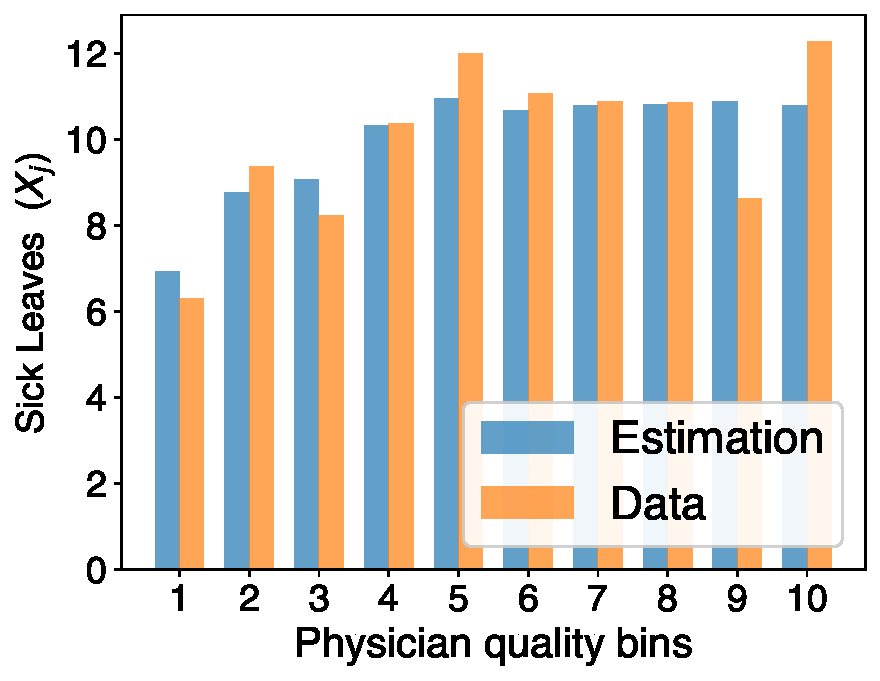
\includegraphics[width=\linewidth]{result_x.pdf}
        
        \caption{$X_j$}

    \end{subfigure}
    \hspace{0.05\linewidth}  % Space between the subfigures
    % Second subfigure
    \begin{subfigure}[b]{0.46\linewidth}
        \centering
        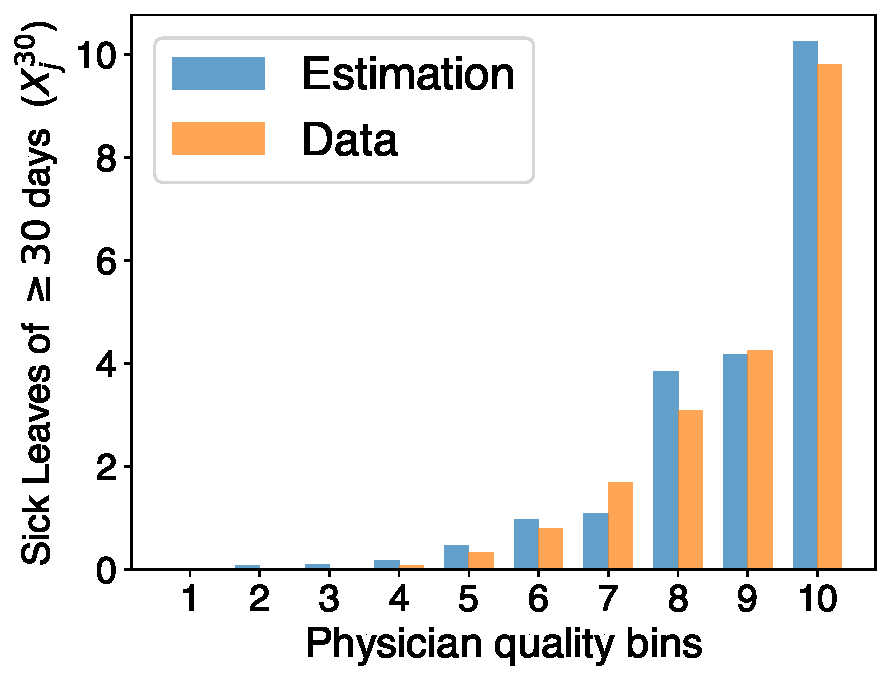
\includegraphics[width=\linewidth]{result_x30.pdf}
        
        \caption{$X_j^{30}$}
    \end{subfigure}


\caption{GMM results \\ Moments by quality bin, Data vs. Model fit (estimation)}
\label{fig:moments}
\end{figure}

The first four representative physicians take a corner, $\kappa_j = 0$ solution. The rest are at the inner solution, satisfying the FOC equation (\ref{eq:ns_FOC}), choosing an increasingly large threshold in relation to their higher $V_j$. Patients satisfying $\kappa_i > \bar{\kappa}_{\max}$, which place high value on physician quality, are concentrated at the highest bins, especially number 10, and they would be even more if were the search parameter $\lambda_s$ were higher.

Even considering the fact that our set-up of physician quality bins amounts to a sort of ``pre-fitting'' of the data to our model, the fitting itself is reasonably succesful, every single one of the twenty moments in the model approaching its data analogue to a high degree, in some cases nearing equality.

\subsection{Identification}

Though fulfilling the minimal condition that we have more equations (20) than moments (15), we need to further ensure the correct identification of each individual parameter. This is straightforward to argue for in the case of the $\vec{V}$ vector, each of the ten $V_j$ parameters directly raises demand for the representative physician $j$, increasing the value of both moments for the respective quality bin. Identification of the other five moments comes from the interplay between the ten $X$ moments and the other ten $X^{30}$ moments.

To get a visual understanding, the Figure \ref{fig:identification} in the Appendix \ref{sec:id} plots the change in the distribution of $X_j$ and $X_j^{30}$ across quality bins for variations in the five remaining parameters. We briefly explain for each parameter the variation in the data which allows for its identification:

\vspace{0.5em}
\begin{xltabular}{\textwidth}{lX}
  
  
    $\lambda_s$ & This parameter determines the ``quality'' of search in the Logit model. As it increases towards $\infty$, demand concentrates exclusively at $V_{10}$. As it tends to 0, demand is uniformly distributed across the ten bins. This sensitivity is more pronounced for the $X^{30}$ moments, sick leaves for patients above $\bar{kappa}_{\max}$, for the reasons mentioned in subsection \ref{sec:moments}: this moment is almost independent from $\gamma_i$, which conversely makes it more sensitive to $V_j$, which is in turn scaled by  $\lambda_s$. This parameter serves to explain, for a given $\vec{V}$, the relative steepness of the distribution of $X^{30}$ with respect to $X$. \\
    \\
    $\bar{\kappa}_{\max}$ & This parameter directly controls the scale of overall $X^{30}$ with respect to $X$. The lower it is, the more aggregate $X^{30}$ approaches aggregate $X$. It should be such that the $X^{30}/X$ ratio resembles the ratio of sick leaves of 30+ days over total sick leaves issued in the data, and indeed it does (21.75\% vs. 20.05\%). \\
    \\
    $p$ & The \textit{punishment} function parameter $p$ determines the level of $X_j$ at which physicians who choose an inner solution $\bar{\kappa_j}$ stay, and the first physician bin which plays an inner solution. Raising or lowering $p$ takes the $X_j$ levels of the six representative physicians of highest quality away from the horizontal they currently occupy, regardless of the magnitude of $V_j$ they hold. \\
    \\
    $\mu, \sigma$ & For these two parameters we run into complications. Jointly, they \textit{can} be identified, as they account for variations in the location of the first inner solution bin beyond what the $p$ parameter can achieve, but they can't be readily separated. The effect of a decrease in $\mu$ is equivalent to that of an \\
    & increase in $\sigma$, furthermore, the distribution is insensitive to an increase in $\mu$ as it is a dicrease in $\sigma$. In this regard we can say that $\mu$ and $\sigma$ jointly describe a feasible plane where the distribution we achieved is possible for values in both parameters, but they fail at reducing this 2-dimensional plane to a singleton, which would be the exact identification of both.
\end{xltabular}

This last result is unfortunate, as it implies we can only \textit{partially} identify the distribution $G(\gamma)$. We nonetheless carry on, but if this issue is to be alleviated, more data moments are to be made available for fitting. It's possible that the mean and variance of $G(\gamma)$ would present heterogenous effects for $Q_j$ as they do on $X_j$, allowing distinction between the two. In that case, data on physicians' clientele would be crucial. Perhaps physician variation across $r_j$ bins would be another solution, rather than our choice of a single $r$ for all. We will touch on this at the end of this paper.

For now, we go on with our estimated parameters and run simulations to showcase our framework.


\section{Counterfactual and Discussion}

With our fitted model at hand, we are in a position to run different scenarios. In particular, what might be the ideal choice of $p$ for the punishment function by a policymaker?

Ideally, a policymaker would be able to stamp out fraud directly, which in our model would imply that they would be able to have direct influence over the physicians' choice of $\bar{\kappa_j}$, namely to place a specified lower bound on it, some level $\underline{\kappa}$ under which patients are under no circumstance to receive sick leave. That is, in a way, the status quo, except for the fact that enforcement is unfeasible. The ``overdetermination'' of roles which \cite{markussen-roed} speak about not only has the consequence that physician serve opposite financial interests (their own and the taxpayers'), but also that, in this occasion, they're better able to cover their tracks. The policymaker, as principal, would like to establish surveillance over their agent, the physician, on whether they've granted unwarranted sick leaves. Only that their only source of information is the agent herself. The agent in charge of diagnosis is the same as then issues sick leave, as such they would have every incentive to fit one to the other, whether legitimately or illegitimately. We mentioned higher scrutiny \textit{does} take place on high duration sick leaves, automatically sent up to the overseer for approval, requiring medical proof. This isn't the case for the routine conditions which make up the majority of observations in our sample, nor would it be practical that it were so.

This isn't necessarily a question of deliberate fraud either. \cite{cln} establish that under all but the most extreme circumstances (read: set of parameters), physicians have no incentive to be distrustful of their patients' self-reported symptoms, whether in fact suspicious of foul play or not. In that regard, our policy of choice would seek to realign the incentives of the physician to that of the policymaker, rather than merely being a question of catching and punishing willing offenders, such that physicians self-police into subjecting diagnosis to some higher level of scrutiny on their part.

Consider for a moment the policymaker \textit{were} able to place restrictions on $\bar{\kappa_j}$. Under our current parameters, if physician strategies, i.e. strictness, were imposed at a fourth of the value of the upper bound, that is, at $\underline{\kappa} = 1/4 \, \bar{\kappa}_{\max}$, total issuance would go down by 32\%. In particular, the lowest 32\% of patients previously receiving sick leave, ordered by their `medical necessity' $\kappa_i$, would be cut off.

How might the policymaker effect such a change through feasible policy means? The careful reader might argue that, in fact, we have already defined the punishment function $P(\cdot)$ as being the purview of the institutional overseer. As misdiagnosis itself isn't observed, punishment takes the form of a probability and magnitude of fine as a function of sick leaves issued over a given period ($X_j$), where we proposed $P(X_j) = p / 2 \cdot (X_j)^2$ as a polynomial approximation. Under this definition, the policymaker would have control over the parameter $p$.

Figure \ref{fig:counter} illustrates the \textit{aggregate} amount of sick leaves issued in the physician-patient market as a function of different relative levels of $p$. The dashed horizontal line is the level of aggregate sick leaves that would be achieved by direct control over physicians' $\bar{\kappa_j}$, placing them at $\underline{\kappa} = 1/4 \, \bar{\kappa}_{\max}$.

\begin{figure}[H]
    \centering
    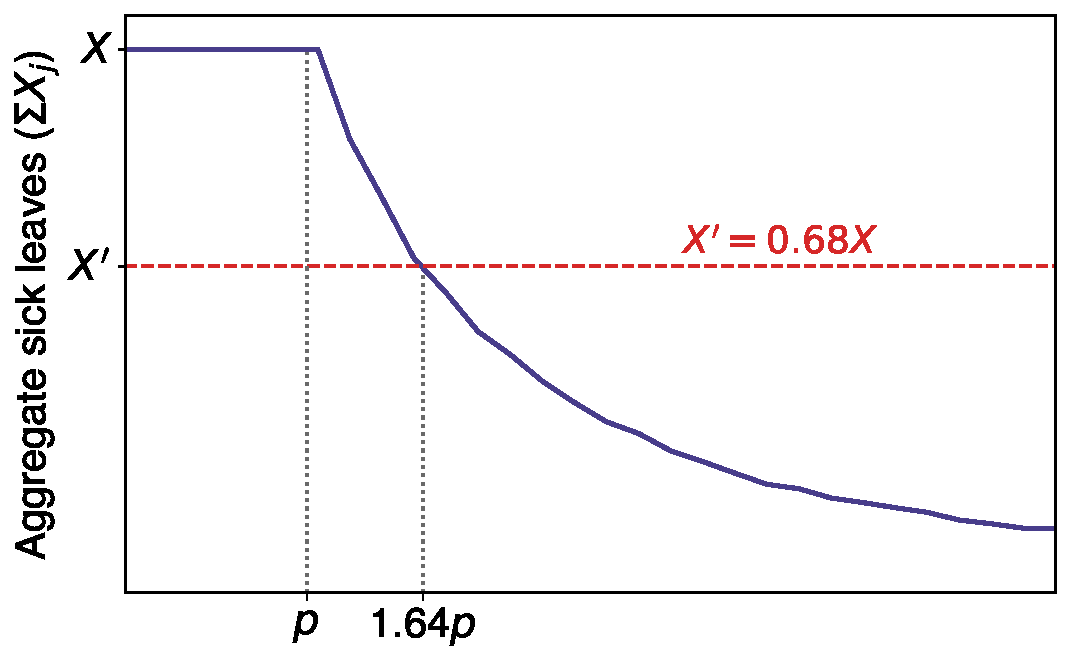
\includegraphics[width=0.60\linewidth]{counter.pdf}
    \captionsetup{justification=centerlast}
    \caption{Aggregate sick leaves in our fitted model for different values of $p$}
    \label{fig:counter}
\end{figure}

We don't directly address the question of welfare in this paper. The optimal choice of $p$, itself informed by the optimal choice of $\underline{\kappa}$, should derive from some model which can numerically formalize its different repercussions. The downside \textit{is} present within our framework itself: raising $p$ presses physicians into higher strictness, reducing overall welfare, as physicians must cut back on their services, facing higher expected penalties for a reduced revenue stream — and patients are in many cases induced to visit lower quality physicians, which decreases their utility with respect to the previous status quo, and are in some cases driven out of the market entirely.

The flipside, the reason why a policimaker would \textit{want} to reduce the issuance of sick leaves, is not present in any shape or form in our framework. These negative consequences are one of the main subjects of the economic literature on sick leaves. Two motives stand out: sick leave fraud puts financial strain on either the taxpayer or employer, whoever covers the worker's wages; and the work absence facilitated by easy access to sick leave has an impact on aggregate productivity. Such effects would need to be included in an estimation of the overall welfare impact of cracking down on sick leave issuance, but they fall well outside of the scope of our analysis.

\section{Conclusion}

We have presented a framework which seeks to include and explain several behaviors in the sick leave market in a parsimonious way: assortative matching of high issuance physicians with high ``usage'' patients, leniency as a response to increasing competition among physicians, heterogenous leniency, imperfect matching. All of these are constructed to be the endogenous outcomes from rational choices by both types of agents, physicians and patients, depending upon certain modelling decisions on our part: heterogenous physicians, fuzzy search, dual source patient utility. In this respect, theoretically, our framework and both its computed specifications give reasonable insight into this market.

As for its use as a guide to policy beyond providing conceptual understanding, that is, correctly predicting the physicians' response to a raise in the probability and/or magnitude of the fine they face for excessive sick leaves granted, its reliability would depend on the plausibility of our chosen functional form for the different distributions and functions and the quality of the data used and performed estimation to calibrate their parameters. It's our view that we achieve the former, but perhaps not the latter. The chosen functional forms are spare in requirements and follow precedents set in the literature. The data we have available, however, is rather thin in comparison to relevant papers on this subject, which affects the quality of our estimation.

As we discussed above, our GMM exercise would benefit greatly from additional sources of information, both in terms of additional variation across physicians, as well as having more parameters be retrieved elsewhere and be set in place by the time we perform estimation, such that we require fewer degrees of freedom. Chief among the possible revisions and extensions to this program: information on the client base of physicians, i.e. a source of $Q_j$, and an alternative, separate method to gauge physician quality, perhaps relating observable qualities like education, tenure, place of work and so on to disagregated data on salaries and visit revenue. Such disaggregated data on its own could prove useful to find more horizontal variation across physicians, setting up bins of $r_j$ and/or $\tau_j$ for their own sake. Ensuring proper identification is foremost among the next steps, but would also require a considerable amount of leg work. \textit{You can only do so much in one semester.}


\end{document}